\documentclass[12pt,letterpaper]{article}
\usepackage[utf8]{inputenc}
\usepackage[spanish]{babel}
\usepackage{graphicx}
\usepackage[left=2cm,right=2cm,top=2cm,bottom=2cm]{geometry}
\usepackage{graphicx} % figuras
% \usepackage{subfigure} % subfiguras
\usepackage{float} % para usar [H]
\usepackage{amsmath}
%\usepackage{txfonts}
\usepackage{stackrel} 
\usepackage{multirow}
\usepackage{enumerate} % enumerados
\renewcommand{\labelitemi}{$-$}
\renewcommand{\labelitemii}{$\cdot$}

% \author{}
% \title{Caratula}
\begin{document}

% Fancy Header and Footer
% \usepackage{fancyhdr}
% \pagestyle{fancy}
% \cfoot{}
% \rfoot{\thepage}
%

% \usepackage[hidelinks]{hyperref} % CREA HYPERVINCULOS EN INDICE

% \author{}
\title{Caratula}

\begin{titlepage}
\begin{center}
\large{UNIVERSIDAD PRIVADA DE TACNA}\\
\vspace*{-0.025in}
\begin{figure}[htb]
\begin{center}

\includegraphics[width=8cm]{./Imagenes/logo}
\end{center}
\end{figure}
\vspace*{0.15in}
INGENIERIA DE SISTEMAS  \\

\vspace*{0.5in}
\begin{large}
TITULO:\\
\end{large}

\vspace*{0.1in}
\begin{Large}
\textbf{INFORME DE LABORATORIO N4 - BI} \\
\end{Large}

\vspace*{0.3in}
\begin{Large}
\textbf{CURSO:} \\
\end{Large}

\vspace*{0.1in}
\begin{large}
INTELIGENCIA DE NEGOCIOS\\
\end{large}

\vspace*{0.3in}
\begin{Large}
\textbf{DOCENTE(ING):} \\
\end{Large}

\vspace*{0.1in}
\begin{large}
 Patrick Cuadros Quiroga\\
\end{large}

\vspace*{0.2in}
\vspace*{0.1in}
\begin{large}
Estudiante: \\
\begin{flushleft}
Salamanca Contreras, Fiorella Rosmery 		\hfill	(2015053237) \\
\end{flushleft}
\end{large}
\end{center}

\end{titlepage}


\tableofcontents % INDICE
\thispagestyle{empty} % INDICE SIN NUMERO
\newpage
\setcounter{page}{1} % REINICIAR CONTADOR DE PAGINAS DESPUES DEL INDICE

\section{Ejercicio N01 - Envíos} 

El siguiente diagrama E / R simplificado describe el envío de mercancías. Los lotes pertenecientes a ciertos grupos se
envían a ciertos destinos en varios países a través de diferentes modos de transporte. Un cierto centro de costos es
responsable de cada envío. La dimensión de tiempo consiste en mes y año.

	\begin{center}
	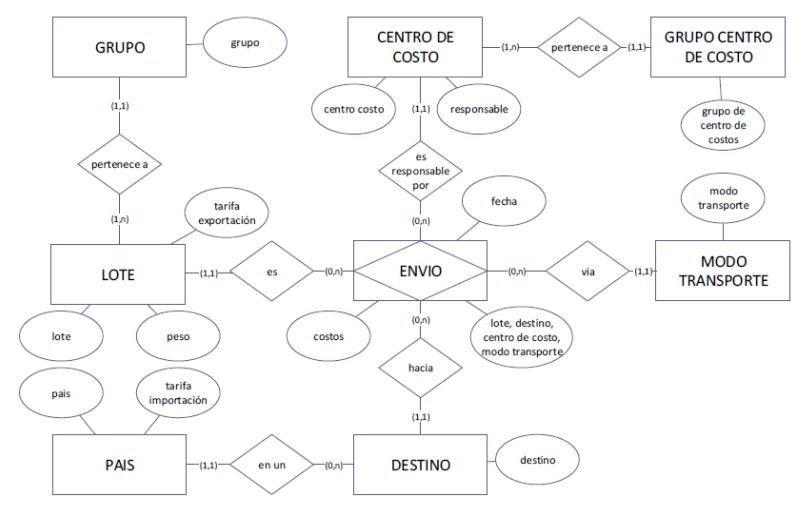
\includegraphics[width=17cm]{./Imagenes/ejercicio1}
	\end{center}	

Supongamos que los costos de los atributos ya incluyen todas las tarifas. No se transferirá más información sobre las tarifas
al almacén de datos. El análisis tendrá lugar a nivel del grupo de centros de costos, no se necesita información sobre los
centros de costos.
Por favor identifique el hecho de interés y construya el Modelo Dimensional y su respectivo diagrama físico.
\\

\begin{itemize}
    \item \textbf{Modelo Dimensional}
\\
El diseñador de software ERWIN permite que se pueda crear y modificar diagramas con facilidad, mejorando la calidad de los diseños de software. El Modelo Dimensional es el resultado directo de la llegada del diseño de flujo de datos y análisis estructural.

	\begin{center}
	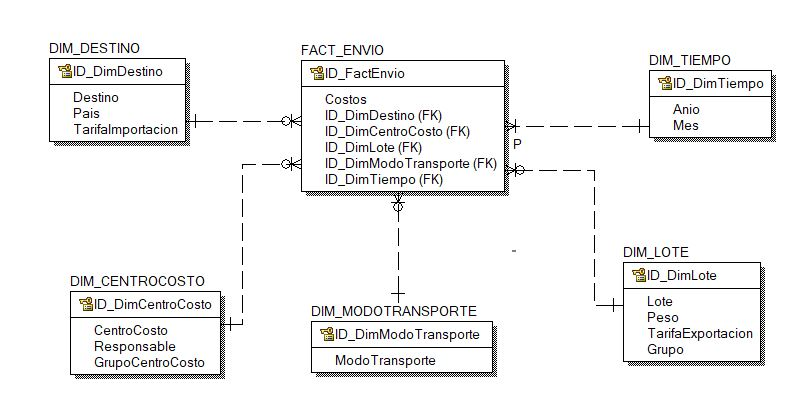
\includegraphics[width=17cm]{./Imagenes/Ejercicio1Logico}
	\end{center}	

    \item \textbf{Modelo Fisico}

Es posible crear y modificar bases de datos de forma visual a través de los diagramas de bases de Datos. Estos diagramas fisicos proporcionan una visión gráfica de las tablas en la base de datos incluyendo sus columnas, el modelo E/R y el diagrama fisico de estructura de datos en SQL Server.

	\begin{center}
	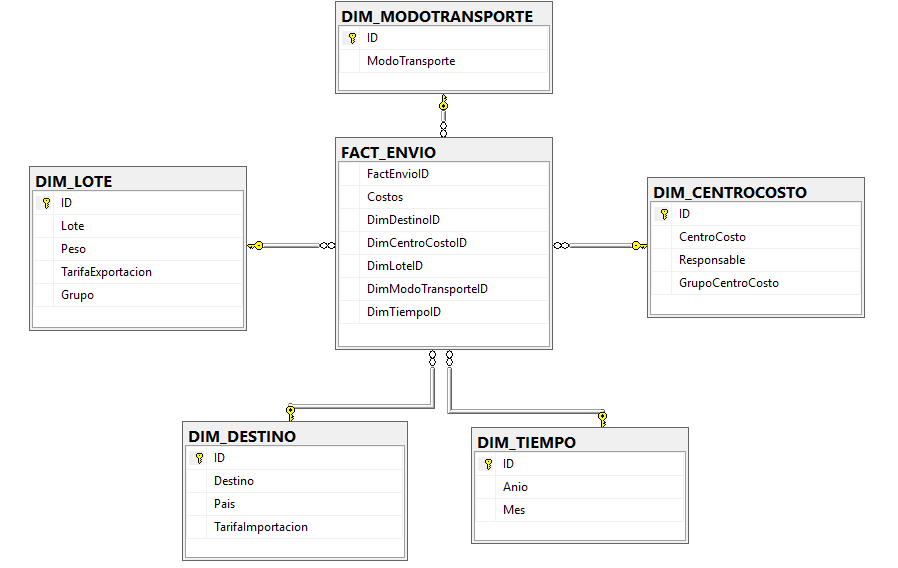
\includegraphics[width=17cm]{./Imagenes/Ejercicio1Fisico}
	\end{center}	

    \item \textbf{Código del Modelo Fisico}

	\begin{center}
	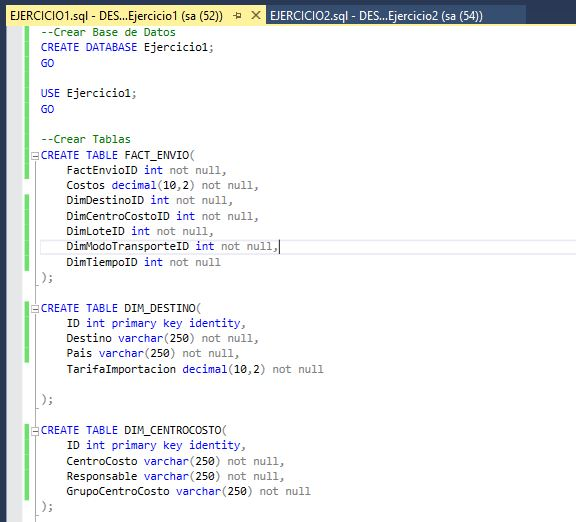
\includegraphics[width=17cm]{./Imagenes/Ejercicio1Fisico1}
	\end{center}	

	\begin{center}
	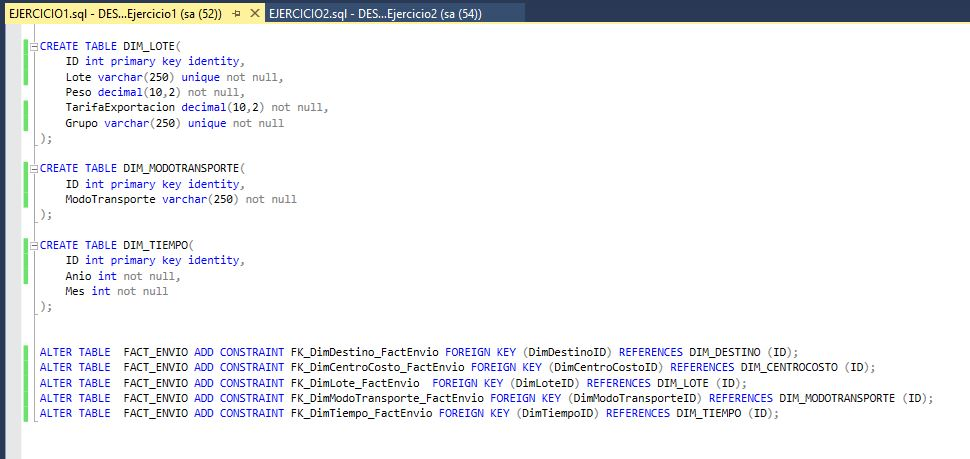
\includegraphics[width=17cm]{./Imagenes/Ejercicio1Fisico2}
	\end{center}	
\end{itemize}
\section{Ejercicio N02 - Reservas de viaje} 

En este esquema de E / R, un cliente (que es de cierto tipo) reserva un viaje en una agencia de viajes. La agencia de viajes
trabaja para un determinado operador turístico. El viaje va a un destino determinado que pertenece a un país determinado.
La dimensión de tiempo consiste en mes, trimestre y año.

	\begin{center}
	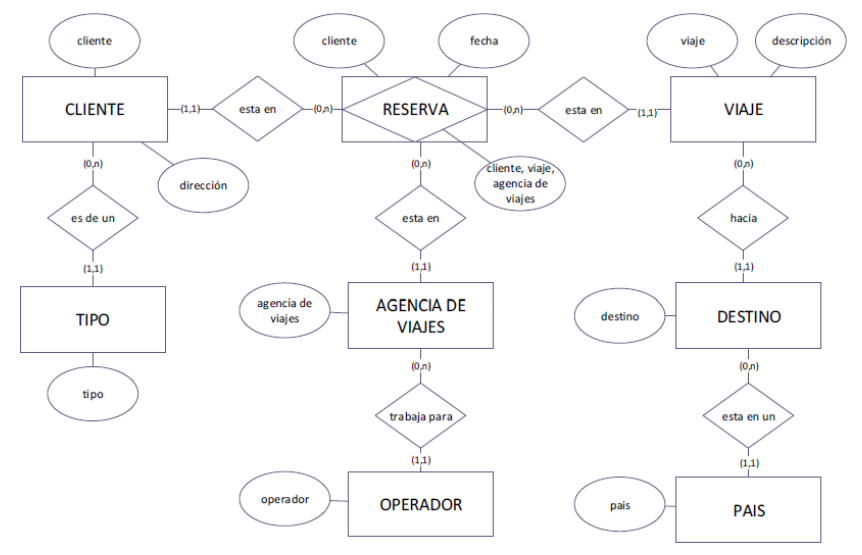
\includegraphics[width=17cm]{./Imagenes/ejercicio2}
	\end{center}	

Por favor identifique el hecho de interés y construya el Modelo Dimensional y su respectivo esquema físico.
\\

\begin{itemize}
    \item \textbf{Modelo Dimensional}
\\
El diseñador de software ERWIN permite que se pueda crear y modificar diagramas con facilidad, mejorando la calidad de los diseños de software. El Modelo Dimensional es el resultado directo de la llegada del diseño de flujo de datos y análisis estructural.

	\begin{center}
	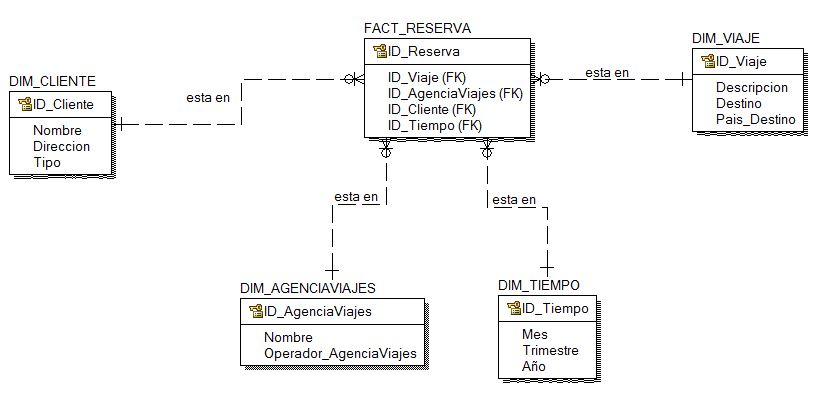
\includegraphics[width=17cm]{./Imagenes/Ejercicio2Logico}
	\end{center}	

    \item \textbf{Modelo Fisico}

Es posible crear y modificar bases de datos de forma visual a través de los diagramas de bases de Datos. Estos diagramas fisicos proporcionan una visión gráfica de las tablas en la base de datos incluyendo sus columnas, el modelo E/R y el diagrama fisico de estructura de datos en SQL Server.

	\begin{center}
	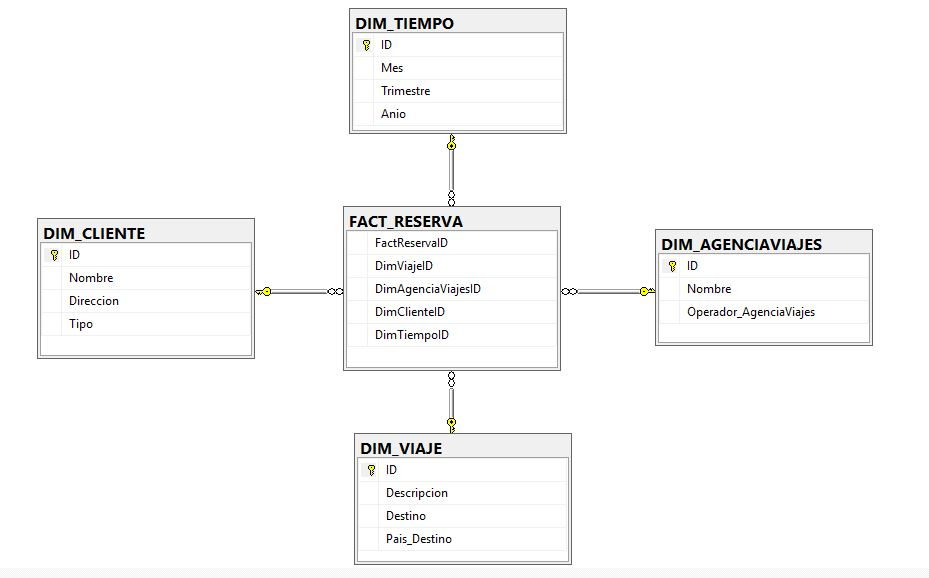
\includegraphics[width=17cm]{./Imagenes/Ejercicio2Fisico}
	\end{center}	

    \item \textbf{Código del Modelo Fisico}

	\begin{center}
	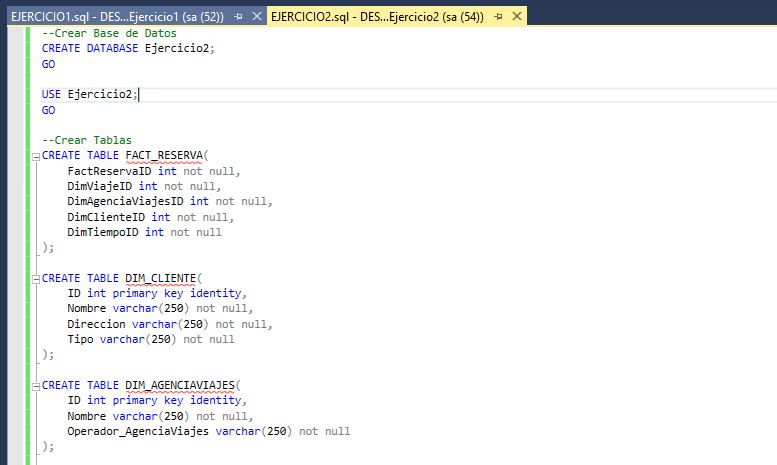
\includegraphics[width=17cm]{./Imagenes/Ejercicio2Fisico1}
	\end{center}	

	\begin{center}
	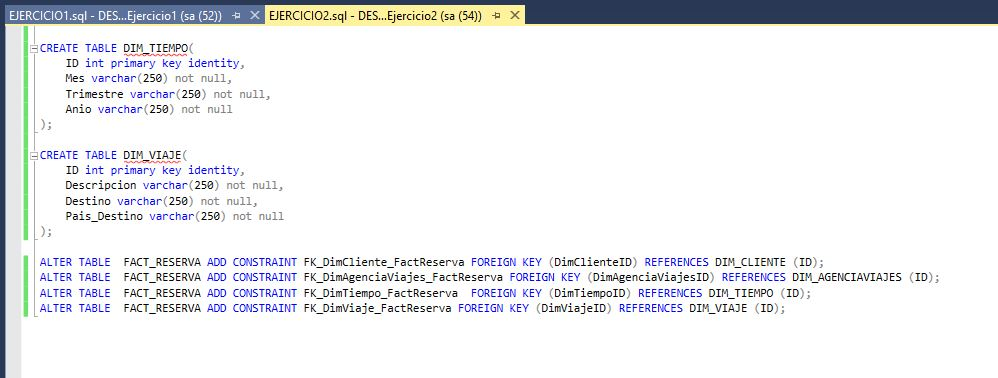
\includegraphics[width=17cm]{./Imagenes/Ejercicio2Fisico2}
	\end{center}	
\end{itemize}
\section{Ejercicio N03 - Gestión de proyectos } 

Este esquema E / R simplificado muestra un caso gestión del proyecto.
El proyecto para un cliente se divide en varios paquetes de trabajo y siempre una persona es responsable de completar la
tarea. Se cuida en un lugar determinado.
La dimensión de tiempo consiste de día, mes y año.


	\begin{center}
	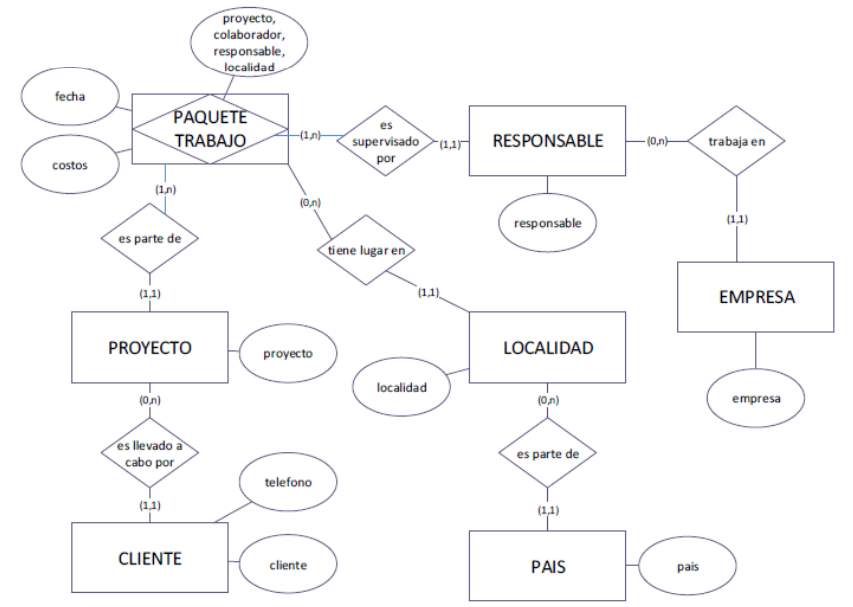
\includegraphics[width=17cm]{./Imagenes/ejercicio3}
	\end{center}	

Por favor identifique el hecho de interés y construya el Modelo Dimensional. Incluya un atributo de hecho adicional que
cuente la cantidad de paquetes de trabajo. Asimismo, realice el diagrama físico.
\\

\begin{itemize}
    \item \textbf{Modelo Dimensional}
\\
El diseñador de software ERWIN permite que se pueda crear y modificar diagramas con facilidad, mejorando la calidad de los diseños de software. El Modelo Dimensional es el resultado directo de la llegada del diseño de flujo de datos y análisis estructural.

	\begin{center}
	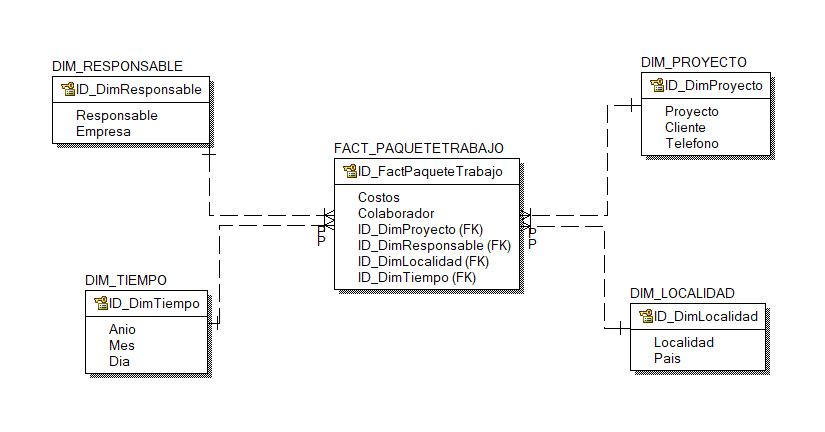
\includegraphics[width=17cm]{./Imagenes/Ejercicio3Logico}
	\end{center}	

    \item \textbf{Modelo Fisico}

Es posible crear y modificar bases de datos de forma visual a través de los diagramas de bases de Datos. Estos diagramas fisicos proporcionan una visión gráfica de las tablas en la base de datos incluyendo sus columnas, el modelo E/R y el diagrama fisico de estructura de datos en SQL Server.

	\begin{center}
	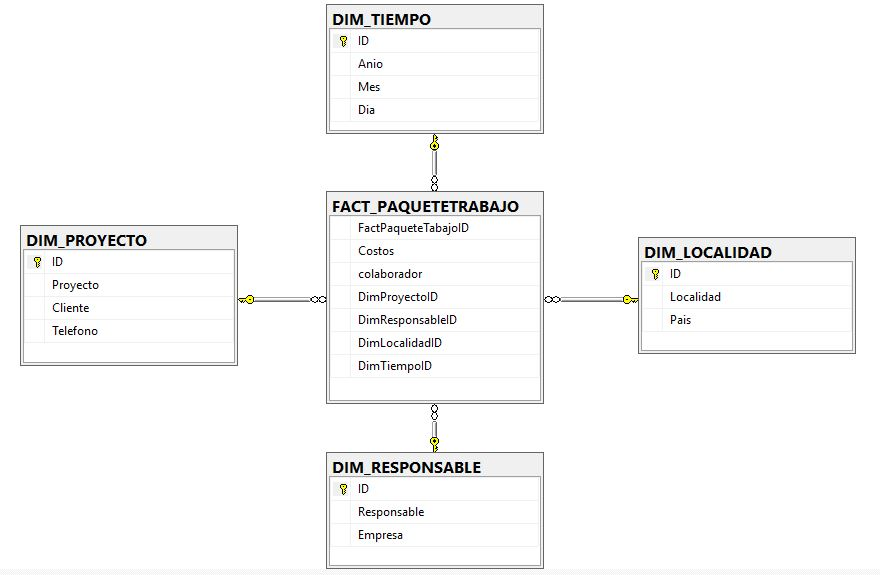
\includegraphics[width=17cm]{./Imagenes/Ejercicio3Fisico}
	\end{center}	

    \item \textbf{Código del Modelo Fisico}

	\begin{center}
	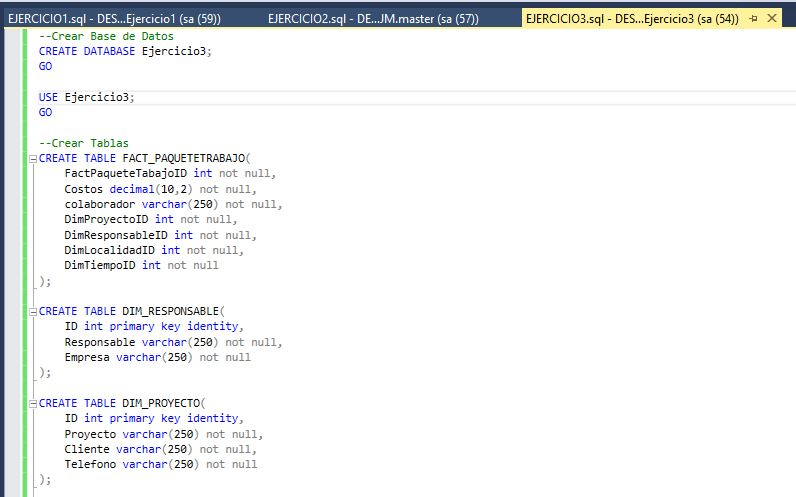
\includegraphics[width=17cm]{./Imagenes/Ejercicio3Fisico1}
	\end{center}	

	\begin{center}
	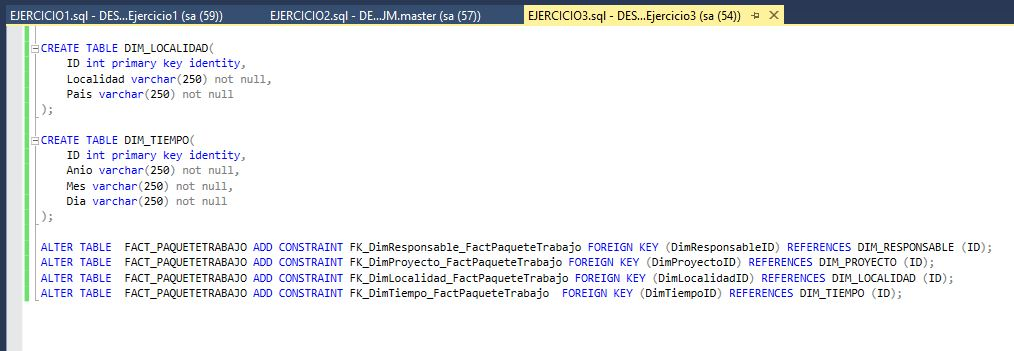
\includegraphics[width=17cm]{./Imagenes/Ejercicio3Fisico2}
	\end{center}	
\end{itemize}

\end{document}
